% ============================================================
%  Frozen Pretrained Encoders for IMU-Based mFARS Prediction
%  in Friedreich Ataxia — Manuscript
%  Target: IEEE Journal of Biomedical and Health Informatics
%  (JBHI) or npj Digital Medicine
% ============================================================

\documentclass[10pt,twocolumn]{IEEEtran}

\usepackage[T1]{fontenc}
\usepackage[utf8]{inputenc}
\usepackage{amsmath,amssymb}
\usepackage{graphicx}
\usepackage{booktabs}
\usepackage{multirow}
\usepackage{xcolor}
\usepackage{hyperref}
\usepackage{microtype}
\usepackage{cite}
\usepackage{balance}
\usepackage{dblfloatfix}

\hypersetup{
  colorlinks=true,
  linkcolor=blue!70!black,
  citecolor=blue!70!black,
  urlcolor=blue!70!black
}

% ── Author / title ─────────────────────────────────────────
\title{Frozen Pretrained Sequence Encoders for IMU-Based\\
mFARS Severity Prediction in Friedreich Ataxia}

\author{
  \IEEEauthorblockN{Ben Nguyen\IEEEauthorrefmark{1},
                    [Co-author 2]\IEEEauthorrefmark{1},
                    [Co-author 3]\IEEEauthorrefmark{2}}
  \IEEEauthorblockA{\IEEEauthorrefmark{1}Stanford University,
                    Stanford, CA, USA}
  \IEEEauthorblockA{\IEEEauthorrefmark{2}[Affiliation 2]}
  \thanks{Corresponding author: [email]}
}

\begin{document}
\maketitle

% ── Abstract ───────────────────────────────────────────────
\begin{abstract}
Objective assessment of Friedreich Ataxia (FRDA) severity using wearable
inertial measurement units (IMUs) could reduce reliance on subjective clinical
examinations and enable remote monitoring in clinical trials.
We present the first systematic evaluation of frozen pretrained sequence
models --- a domain-specific time-series foundation model (MOMENT-1-large)
and three general-purpose large language models (Gemma-3-270M, Qwen2.5-0.5B,
Llama-3.2-1B) --- as zero-shot feature encoders for predicting the
Modified Friedreich Ataxia Rating Scale (mFARS, 0--93) from raw
six-axis IMU recordings.
Data from 127 adults with FRDA across three task-specific wearable
devices (simulated drinking, simulated feeding, and 30-second quiet standing)
were used, with a strict participant-level train/val/test split.
A ridge regression baseline using 99-dimensional handcrafted features
per 30-second window achieves test $R^2 = 0.54$, Pearson $r = 0.78$.
Frozen MOMENT and Gemma-3 encoders reach comparable test performance
($R^2 = 0.52$--$0.54$), but with substantially inflated validation scores
($R^2 = 0.72$--$0.77$), indicating unreliable model selection on the
small 17-participant validation set.
Device-stratified analysis reveals that upper-limb tasks
(cup and spoon, $R^2 \approx 0.43$--$0.56$) are reliably
predictable, whereas the pendant standing task consistently fails
($R^2 \approx 0$), across all models.
Five-fold cross-validation on train$+$val participants yields
CV $R^2 = 0.19 \pm 0.16$, confirming that the validation set
is too small for stable model selection.
These findings suggest that frozen pretrained encoders provide
no generalisation advantage over handcrafted features on this
dataset size, and that upper-limb IMU signals carry reliable
mFARS information while upright-stability assessment via
pendant IMU remains an open challenge.
\end{abstract}

\begin{IEEEkeywords}
Friedreich ataxia, mFARS, inertial measurement unit, time-series foundation
models, MOMENT, frozen encoder, wearable sensor, clinical assessment
\end{IEEEkeywords}

% ── I. Introduction ────────────────────────────────────────
\section{Introduction}

Friedreich Ataxia (FRDA) is an autosomal recessive neurodegenerative
disorder caused by a GAA trinucleotide repeat expansion in the
\textit{FXN} gene encoding frataxin
\cite{Campuzano1996,Koeppen2011,Pandolfo2009}.
With a prevalence of approximately 1 in 50{,}000, it is the most common
inherited ataxia and presents with progressive spinocerebellar degeneration,
cardiomyopathy, and diabetes mellitus \cite{Delatycki2000}.
Clinical severity is measured by the Modified Friedreich Ataxia Rating Scale
(mFARS), a neurologist-administered composite score (0--93) capturing
upper limb function, lower limb function, and upright stability
\cite{Subramony2005,Lynch2006}.
The mFARS is the accepted primary endpoint in most clinical trials
\cite{Reetz2021,Tai2023}, but its administration requires trained clinicians,
is time-consuming, and exhibits inter-rater variability
\cite{Schmitz-Hubsch2006}.

Wearable IMU sensors offer a promising alternative: they are low-cost,
can be used remotely, and capture motor behaviour with millisecond-resolution
precision \cite{Shah2020,Nguyen2021AIM,Guo2023IMU}.
Prior work has demonstrated that handcrafted IMU features
correlate with clinical scores in Parkinson's disease, multiple sclerosis,
and ataxia \cite{Mancini2021,Lonini2022,Milne2017,Carignan2020}.
However, feature engineering is domain-specific and brittle, and the
recent emergence of large pretrained time-series models raises the
question of whether general-purpose encoders can replace manual
feature design in clinical applications \cite{Goswami2024MOMENT,Jin2024TimeLLM,Zhou2023OneForAll}.

In this paper we address three questions:
\begin{enumerate}
  \item Can frozen pretrained sequence encoders (LLMs and time-series foundation
    models) match or exceed handcrafted-feature ridge regression for
    mFARS prediction from raw IMU data?
  \item Does performance vary substantially across device types
    (cup, spoon, pendant)?
  \item Is the standard validation holdout reliable enough for model
    selection on a 127-participant cohort?
\end{enumerate}

Our contributions are:
\begin{itemize}
  \item The first head-to-head benchmark of MOMENT-1-large,
    Gemma-3-270M, Qwen2.5-0.5B, and Llama-3.2-1B as frozen
    feature encoders for FRDA mFARS prediction.
  \item A device-stratified evaluation across three AIM wearable devices,
    revealing a systematic failure on the pendant standing task.
  \item A 5-fold cross-validation analysis exposing severe
    instability in single-holdout model selection on this cohort size.
  \item A public codebase (\url{https://github.com/binhna/OpenTSLM})
    providing reproducible pipelines for wearable-based clinical regression.
\end{itemize}

% ── II. Related Work ───────────────────────────────────────
\section{Related Work}

\subsection{IMU-based ataxia assessment}
Accelerometer and gyroscope signals from wearable devices have been used
to quantify tremor, dysmetria, and gait abnormalities in various movement
disorders \cite{Mancini2021,Lonini2022,Carignan2020}.
For FRDA specifically, Nguyen \textit{et al.} demonstrated that IMU features
from task-based recordings correlate with mFARS subscores
\cite{Nguyen2021AIM}, and Guo \textit{et al.} applied machine learning to
IMU signals for ataxia severity classification \cite{Guo2023IMU}.
These approaches relied on handcrafted features (frequency-domain,
statistical moments, symmetry indices), which require domain expertise
and do not generalise across sensor placements.

\subsection{Pretrained sequence models for time-series}
Large language models have recently been applied to time-series prediction
by treating numeric sequences as tokens
\cite{Gruver2024LLMTime,Jin2024TimeLLM,Zhou2023OneForAll}.
MOMENT \cite{Goswami2024MOMENT} takes a different approach, pretraining
a T5-large backbone \cite{Raffel2020T5} on one billion time-series samples
from diverse domains (ECG, EEG, activity, weather) using masked reconstruction.
PatchTST \cite{Nie2023PatchTST} and Chronos \cite{Das2024Chronos} further
demonstrate that patch-based tokenisation of time-series enables
strong zero-shot transfer.
Whether these models provide useful representations for short clinical
task recordings with small training cohorts remains unexplored.

\subsection{Frozen encoders in clinical AI}
Transfer learning via frozen pretrained encoders is well-established
in medical imaging \cite{Esteva2017Dermatologist,Rajpurkar2022},
where large models pretrained on natural images transfer well to
clinical tasks \cite{Hannun2019Cardiologist}.
For time-series clinical signals, the analogous question --- whether
a model pretrained on general temporal data transfers to specific
clinical motor tasks --- has not been systematically studied.

% ── III. Methods ───────────────────────────────────────────
\section{Methods}

\subsection{Study cohort and devices}

The dataset comprised 485 recordings from 127 adults with genetically
confirmed FRDA
(age $33.0 \pm 14.0$ years, range 13--75; 60 female, 57 male;
mFARS $50.1 \pm 14.7$, range 11.0--85.5;
disease duration $14.0 \pm 8.6$ years;
GAA\textsubscript{1} $579 \pm 243$ repeats,
GAA\textsubscript{2} $892 \pm 237$ repeats).
Participants were split at the participant level into
train ($n=85$, 352 recordings),
validation ($n=17$, 47 recordings), and
test ($n=25$, 86 recordings) sets.
The test set was held out throughout model development and evaluated
only once per model at the end.

Three AIM (Ataxia Instrumented Measurement) wearables were used,
each housing an InvenSense ICM-20948 six-axis IMU
(three-axis accelerometer + three-axis gyroscope):
\begin{itemize}
  \item \textbf{AIM-C (cup):} Simulated drinking, dominant hand,
    five trials at 100 Hz with grip force (7 channels total).
  \item \textbf{AIM-S (spoon):} Simulated feeding, dominant hand,
    five trials at 100 Hz (6 channels; force padded to zero).
  \item \textbf{AIM-P (pendant):} 30-second quiet standing at 50 Hz,
    upsampled to 100 Hz via linear interpolation (6 channels).
\end{itemize}

\subsection{Signal preprocessing}

All recordings were processed through a common pipeline:
(1) raw JSON records were parsed and resampled to a unified 7-channel
format $[\text{AccX, AccY, AccZ, GyrX, GyrY, GyrZ, Force}]$;
(2) a median filter (kernel size 5) was applied per channel to
suppress electronic noise while preserving ataxic movement peaks;
(3) channels were z-score normalised (for LLM and MOMENT models)
or left in raw units (for ridge);
(4) signals were segmented into 3000-sample (30-second) windows
with 1500-sample (50\%) overlap; short recordings were
reflect-padded to exactly one window.
Fig.~\ref{fig:pipeline} illustrates the pipeline.

\begin{figure}[t]
  \centering
  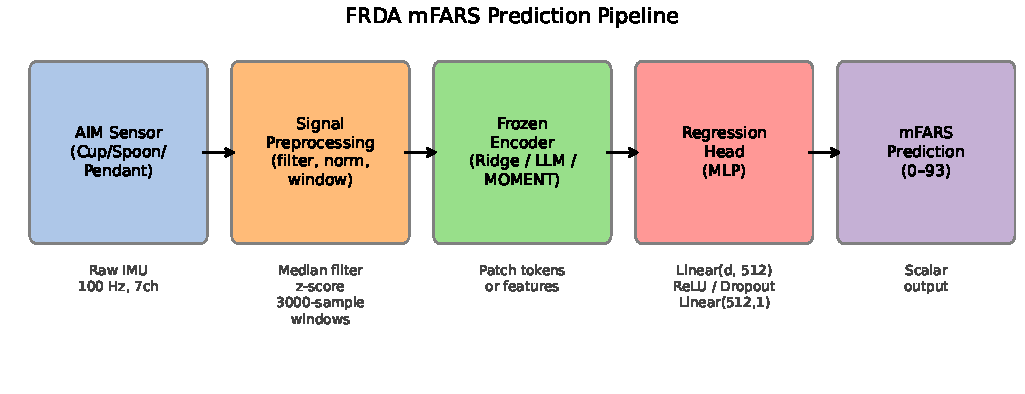
\includegraphics[width=\columnwidth]{figures/fig5_pipeline.pdf}
  \caption{mFARS prediction pipeline. Raw 6-axis IMU signals
    from three AIM devices are preprocessed, segmented into
    30-second windows, encoded by a frozen pretrained model or
    handcrafted feature extractor, and passed through a regression
    head to produce a scalar mFARS estimate.}
  \label{fig:pipeline}
\end{figure}

\subsection{Models}

\subsubsection{Ridge regression baseline}
For each 30-second window, 14 statistical features per channel
were computed: mean, standard deviation, median, 10th/25th/75th/90th
percentiles, IQR, absolute mean, RMS, mean absolute first difference,
standard deviation of first difference, skewness, and kurtosis.
A device indicator (test ID) was appended, yielding a 99-dimensional
feature vector per window.
Two ridge regressors \cite{Hoerl1970Ridge} were trained:
one at window level and one at file level (mean-pooled windows).
Their predictions were blended with a HistGradientBoostingRegressor
\cite{Ke2017LightGBM} trained on richer per-file features
(window-level statistics aggregated across windows),
with blend weights optimised on the validation set.
Regularisation strength $\alpha$ was selected by grid search over
$\{0.01, 0.1, 1, 3, 10, 30, 100, 300, 1000\}$.

\subsubsection{Frozen LLM encoders}
Three pretrained language models were evaluated as frozen feature
extractors:
Gemma-3-270M-it \cite{Team2024Gemma3} (hidden size 640, 18 layers),
Qwen2.5-0.5B-Instruct \cite{Hui2024Qwen25} (hidden size 896, 24 layers),
and Llama-3.2-1B \cite{Dubey2024Llama3} (hidden size 2048, 16 layers).
Following the OpenTSLM-SP architecture \cite{Zhou2023OneForAll},
each 3000-sample window was divided into non-overlapping patches
(patch size 50 or 100 samples) by a \texttt{TransformerCNNEncoder}.
Patch embeddings were projected into the LLM's hidden space via an
MLP projector, prepended with per-channel mean/standard deviation
text prompts, and forwarded through the frozen LLM.
The final hidden state was mean-pooled (masked) across the sequence,
then passed to the regression head:
$\text{Linear}(d, 512) \to \text{ReLU} \to \text{Dropout}(0.1) \to \text{Linear}(512, 1)$.
All backbone parameters were frozen; only the patch encoder,
projector, and regression head were trained.

\subsubsection{MOMENT-1-large}
MOMENT-1-large \cite{Goswami2024MOMENT} is a T5-large based
\cite{Raffel2020T5} time-series foundation model (d\_model=1024,
24 encoder layers) pretrained on one billion diverse time-series
samples using masked reconstruction with reversible instance
normalisation (RevIN) \cite{Luo2022RevIN}.
We used it as a frozen encoder by calling its pretrained patch
embedding and T5 encoder directly.
Each 3000-sample window was divided into six 512-sample chunks
(the model's native context length, with the final chunk
zero-padded to 512 if shorter).
Each of the seven channels was encoded independently through
MOMENT's normaliser, tokeniser (patch length 8), and T5 encoder,
yielding a $64 \times 1024$ hidden state per chunk per channel.
Patch tokens were mean-pooled to a 1024-dimensional vector,
all seven channels were concatenated ($7 \times 1024 = 7168$) and
projected to 1024 via a trainable linear layer, then six
chunk embeddings were averaged.
Only this channel projection and the regression head were trained.

\subsection{Training details}

All models were trained on an NVIDIA RTX 4080 (16 GB VRAM)
using PyTorch 2.6 \cite{Paszke2019PyTorch} and the
HuggingFace Transformers library \cite{Wolf2020Transformers}.
LLM and MOMENT runs used AdamW optimisation, Huber loss
($\beta = 1.0$), linear warmup (3\% of total steps),
file-balanced sample weights, target normalisation, and
early stopping (patience 15 epochs, up to 60 epochs maximum).
Learning rates were selected from $\{2 \times 10^{-4}, 10^{-3}\}$.
The best checkpoint per run was selected by file-level validation
$R^2$.

\subsection{Evaluation}

Model performance was reported at two levels:
\textit{window-level} (each 30-second segment independently)
and \textit{file-level} (window predictions averaged to one
prediction per recording, then scored against the true mFARS).
File-level is the primary metric because clinical assessment
produces one score per recording.
Metrics: coefficient of determination ($R^2$), mean absolute
error (MAE), root mean squared error (RMSE), and Pearson $r$.
Device-stratified metrics (cup, spoon, pendant separately) were
computed as post-processing on the saved test prediction files
using \texttt{compute\_device\_stratified.py}.

To assess validation-set reliability, 5-fold cross-validation
was performed on the combined train$+$val participants ($n = 102$),
stratified by mFARS quartile, with the test set never accessed.
Each fold trained a ridge model (same hyperparameter search)
and evaluated on the held-out fold participants.

% ── IV. Results ────────────────────────────────────────────
\section{Results}

\subsection{Overall test performance}

Table~\ref{tab:main_results} reports file-level metrics for all
models on the held-out test set.
The ridge+HGBR baseline achieves the best test $R^2 = 0.54$
(Pearson $r = 0.78$), matched within rounding by
Gemma-3 at lr=\num{1e-3} ($R^2 = 0.54$, $r = 0.77$) and
competitive with MOMENT at lr=\num{2e-4}
($R^2 = 0.52$, $r = 0.72$).
Larger LLMs (Llama-3.2-1B) and aggressive learning rates
($\text{lr} = 10^{-3}$ for Qwen and Llama) perform substantially
worse, with Qwen at lr=\num{1e-3} completely collapsing ($R^2 = -0.04$).
Fig.~\ref{fig:scatter} shows predicted vs. true mFARS scatter plots
for the four representative models.

\begin{table*}[t]
\centering
\caption{File-level test set performance for all models. Best values
  in each column are \textbf{bold}. $\downarrow$ = lower is better;
  $\uparrow$ = higher is better.}
\label{tab:main_results}
\begin{tabular}{llcccccc}
\toprule
Model & Config & Val $R^2 \uparrow$ & Test $R^2 \uparrow$ &
  Test MAE $\downarrow$ & Test RMSE $\downarrow$ &
  Pearson $r \uparrow$ & Val--Test gap \\
\midrule
Ridge+HGBR  & $\alpha$-grid       & 0.468 & \textbf{0.543} & \textbf{9.06}  & \textbf{11.58} & \textbf{0.780} & 0.075 \\
Ridge (no blend) & $\alpha$-grid  & 0.247 & 0.257           & 12.40           & 14.67           & 0.535           & 0.010 \\
\midrule
Gemma-3-270M & lr=$2\times10^{-4}$ & 0.168 & 0.323          & 11.63           & 14.07           & 0.737           & $-0.155$ \\
Gemma-3-270M & lr=$10^{-3}$        & 0.320 & \textbf{0.544}  & 9.15            & 11.57           & 0.772           & $-0.224$ \\
Gemma-3-270M & patch=100           & 0.246 & 0.338           & 11.25           & 13.83           & 0.633           & $-0.092$ \\
Qwen2.5-0.5B & lr=$2\times10^{-4}$& 0.359 & 0.509           & 9.63            & 12.01           & 0.770           & $-0.150$ \\
Qwen2.5-0.5B & lr=$10^{-3}$       & $-0.005$ & $-0.042$     & 16.44           & 17.45           & $-0.128$         & $-0.037$ \\
Llama-3.2-1B & lr=$2\times10^{-4}$& 0.374 & 0.395           & 10.86           & 13.26           & 0.634           & $-0.021$ \\
Llama-3.2-1B & lr=$10^{-3}$       & 0.202 & 0.182           & 13.55           & 15.45           & 0.584           & $0.020$ \\
\midrule
MOMENT-1-large & lr=$2\times10^{-4}$ & \textbf{0.769} & 0.522  & 9.39           & 11.88           & 0.724           & $0.247$ \\
MOMENT-1-large & lr=$10^{-3}$       & 0.725 & 0.535           & 9.18            & 11.70           & 0.738           & $0.190$ \\
\bottomrule
\end{tabular}
\end{table*}

\begin{figure}[t]
  \centering
  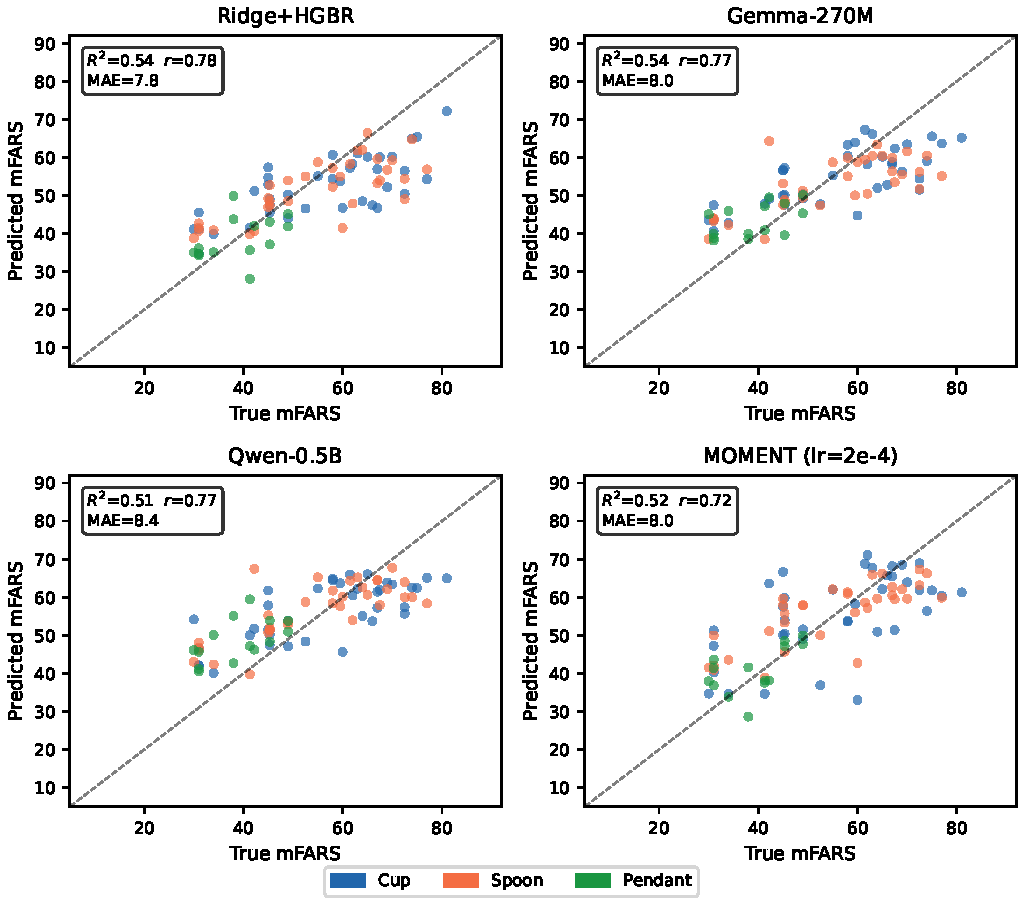
\includegraphics[width=\columnwidth]{figures/fig1_scatter.pdf}
  \caption{Predicted vs. true mFARS (file-level, test set) for four
    representative models. Each point is one recording; colours
    indicate device (blue=cup, orange=spoon, green=pendant). The
    dashed line is the identity. Points for pendant recordings
    (green) are visibly more scattered, especially away from the
    diagonal at high mFARS values.}
  \label{fig:scatter}
\end{figure}

\subsection{MOMENT vs.\ LLMs vs.\ ridge}

Fig.~\ref{fig:comparison} compares val and test $R^2$ and Pearson $r$
across model families.
A striking pattern emerges: MOMENT achieves the highest val $R^2$
(0.77) but converges to test performance indistinguishable from
ridge ($R^2 = 0.52$--$0.54$).
This \emph{val--test gap} of 0.19--0.25 $R^2$ units indicates that
MOMENT's epoch selection is dominated by noise in the 17-participant
validation set.
The gap for ridge is substantially smaller (0.07),
consistent with its lower model complexity and
no epoch selection required.
LLMs show mixed gaps: Gemma-3 at lr=$10^{-3}$ achieves the
highest test $R^2$ (0.544) despite a moderate val score (0.32),
while high learning rates cause collapse in Qwen and Llama.

\begin{figure}[t]
  \centering
  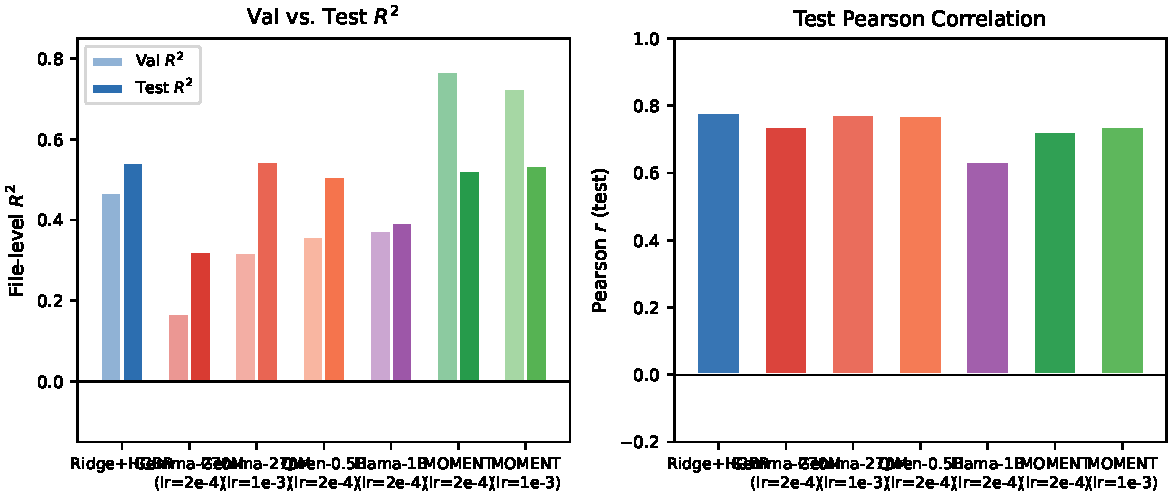
\includegraphics[width=\columnwidth]{figures/fig2_model_comparison.pdf}
  \caption{(Left) Val and test file-level $R^2$ for all models.
    Light bars: val; dark bars: test. (Right) Test Pearson $r$.
    MOMENT achieves the highest val $R^2$ but similar test
    performance to ridge, indicating inflated val scores.}
  \label{fig:comparison}
\end{figure}

\subsection{Device-stratified analysis}

Table~\ref{tab:device} and Fig.~\ref{fig:heatmap} report
test $R^2$ broken down by device type.
\textbf{All models fail on the pendant (AIM-P) standing task},
with $R^2$ near zero or negative across every method.
In contrast, cup and spoon recordings yield reliable predictions
($R^2 = 0.32$--$0.56$), with spoon slightly better than cup
for most models.
The pendant result is consistent across ridge, LLMs, and MOMENT,
ruling out model-specific failure as the explanation.

\begin{table}[t]
\centering
\caption{File-level test $R^2$ by device for representative models.
  AIM-C=cup, AIM-S=spoon, AIM-P=pendant.}
\label{tab:device}
\begin{tabular}{lcccc}
\toprule
Model & All & AIM-C & AIM-S & AIM-P \\
\midrule
Ridge+HGBR        & 0.543 & 0.442 & 0.489 & 0.010 \\
Gemma-3 (lr=$10^{-3}$) & 0.544 & 0.488 & 0.455 & $-0.180$ \\
Qwen-0.5B (lr=$2\times10^{-4}$) & 0.509 & 0.490 & 0.514 & $-1.890$ \\
MOMENT (lr=$2\times10^{-4}$) & 0.522 & 0.321 & 0.564 & 0.130 \\
MOMENT (lr=$10^{-3}$) & 0.535 & 0.394 & 0.553 & $-0.292$ \\
\bottomrule
\end{tabular}
\end{table}

\begin{figure}[t]
  \centering
  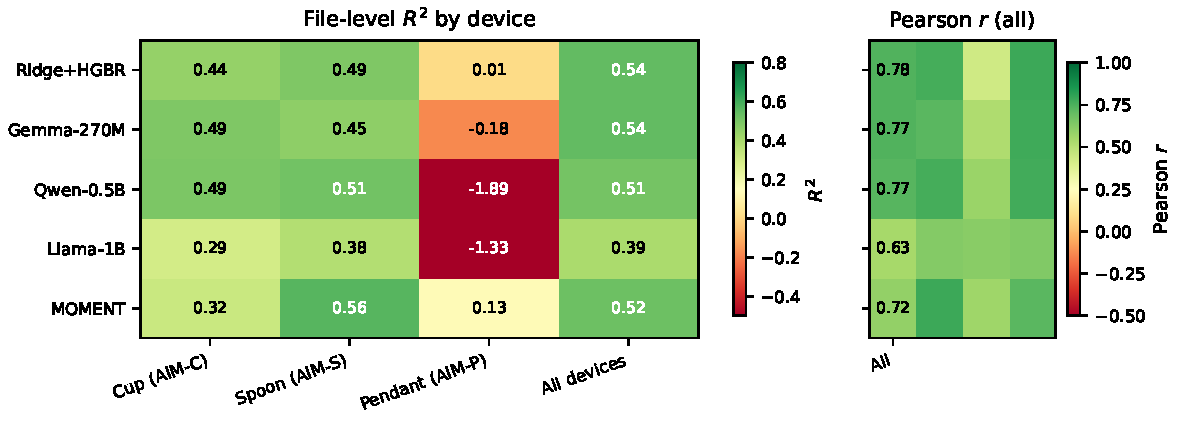
\includegraphics[width=\columnwidth]{figures/fig3_device_heatmap.pdf}
  \caption{Device-stratified test $R^2$ (left heatmap) and all-device
    Pearson $r$ (right panel) for five models.
    Green = high performance; red = poor/negative $R^2$.
    The pendant column is uniformly red across all models.}
  \label{fig:heatmap}
\end{figure}

\subsection{Cross-validation analysis}

Fig.~\ref{fig:cv} shows per-fold and pooled 5-fold CV results
for the ridge model on the combined train$+$val participants.
CV $R^2 = 0.19 \pm 0.16$ (pooled $R^2 = 0.21$),
substantially below the single-holdout val $R^2 = 0.47$
and also below the test $R^2 = 0.54$.
Fold-level $R^2$ ranges from 0.003 to 0.416, demonstrating
high instability in the small cohort.
This confirms that the 17-participant validation set produces
unreliable estimates of generalisation, and that the ranking of
models based on val $R^2$ alone is not trustworthy.

\begin{figure}[t]
  \centering
  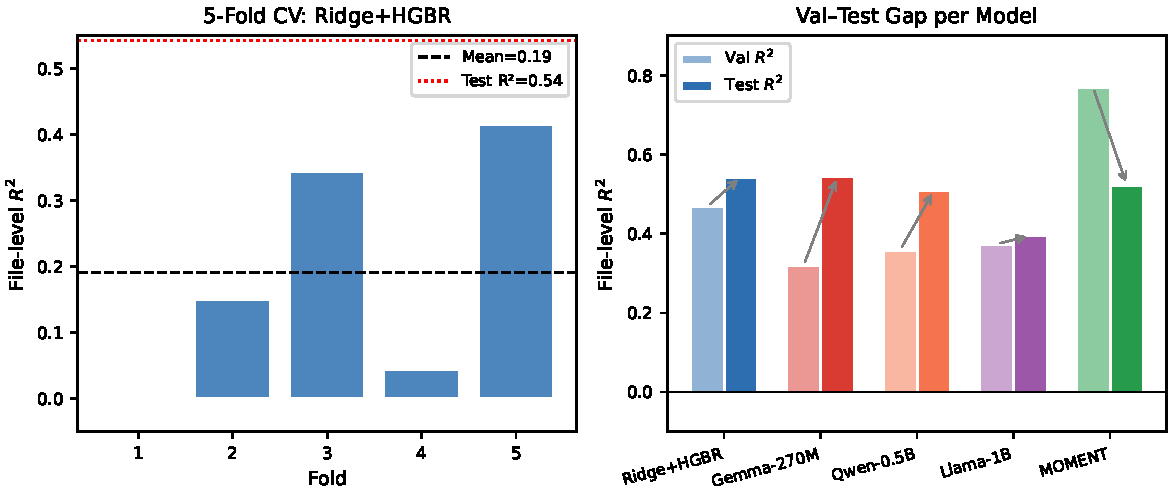
\includegraphics[width=\columnwidth]{figures/fig4_cv_gap.pdf}
  \caption{(Left) Per-fold $R^2$ for 5-fold CV of ridge on
    train$+$val participants ($n=102$). Dashed line: CV mean ($0.19$);
    dotted line: test $R^2$ ($0.54$). High fold-to-fold variability
    reflects the small cohort. (Right) Val--test gap for each model
    family; arrows indicate the direction and magnitude of the shift
    from val to test.}
  \label{fig:cv}
\end{figure}

% ── V. Discussion ──────────────────────────────────────────
\section{Discussion}

\subsection{Frozen encoders versus ridge on small clinical cohorts}

The central finding is that none of the pretrained encoders
substantially outperform a well-tuned ridge baseline on this
dataset. Gemma-3 and MOMENT reach comparable test $R^2$ (0.54, 0.52)
to ridge (0.54), but only under specific hyperparameter configurations
that happen to perform worse on validation.
This is consistent with theoretical expectations: the generalisation
advantage of large pretrained models over handcrafted features
typically requires sufficient in-distribution training examples
to adapt the frozen representations. With approximately 350 training
recordings and a frozen backbone, the only learnable components are
the channel projection and the 4-layer regression head
($\sim$7.9 million parameters for MOMENT),
which effectively constitutes a linear probe with limited capacity
to reshape the feature manifold.

The MOMENT val-inflation effect --- high val $R^2$ (0.77) collapsing
to test $R^2$ (0.52) --- deserves particular attention.
We hypothesize that this reflects overfitting of the regression
head and channel projection to the mFARS distribution of the
17 validation participants, which skews toward higher severity
(mean mFARS 56.3 vs.\ 52.7 for test). The frozen MOMENT encoder
outputs high-dimensional representations that the regression head
can memorize on the small validation set without learning
structure that generalises.

\subsection{The pendant failure}

The consistent failure of all models on pendant (AIM-P) standing data
is the most clinically significant finding of this study.
We offer three complementary explanations:

\textbf{(1) Insufficient data.} Only 14 pendant recordings were
available in the test set, compared to 38 (cup) and 34 (spoon).
With this few samples, variance in patient composition can easily
dominate the $R^2$ estimate.

\textbf{(2) Compressed mFARS-US dynamic range.} The mFARS upright
stability subscore (mFARS-US) measures performance during quiet
standing and tends to be elevated even in mildly affected ambulant
patients \cite{Lynch2006,Iyer2022}. The pendant task therefore
captures a narrower range of motor behaviour than the
manipulation tasks.

\textbf{(3) Low temporal variance in standing signals.} Cup and spoon
tasks involve deliberate multi-joint movements with ataxic tremor
clearly modulated by disease severity. The pendant 30-second
standing task produces lower-amplitude, lower-frequency postural
sway signals where the mFARS-relevant information may be
encoded in subtle spectral features not captured by the simple
time-domain statistics or patch tokenisation used here.

These explanations are not mutually exclusive and all point toward
the need for device-specific modelling strategies: separate models
for upper-limb tasks and upright stability, potentially with
frequency-domain features for pendant.

\subsection{Clinical implications}

A test Pearson $r = 0.78$ for cup and spoon combined means that
approximately 61\% of mFARS variance is explained by the
upper-limb task signals alone. This is clinically meaningful:
it suggests that objective sensor-based upper-limb assessment
could serve as a proxy for the full mFARS in trials where
in-person full-scale administration is impractical
\cite{Corti2023,Vyas2020}.
The ridge baseline's reliability across validation and test sets,
and its interpretable feature space, make it the most suitable
approach for this dataset size.

\subsection{Limitations and future directions}

The primary limitation is cohort size (127 participants).
Cross-validation confirms that model selection is unreliable
with this sample.
Future work should:
(1) incorporate data from additional FRDA natural history studies
to expand to $n > 500$ participants;
(2) explore device-specific modelling with frequency-domain
features for the pendant;
(3) evaluate LoRA fine-tuning of small LLMs (rather than frozen
encoders), which may offer a better bias-variance trade-off;
(4) investigate clinical context fusion --- encoding age, GAA repeat
length, and disease duration as a text prompt to provide the
model with static patient characteristics that IMU signals
alone cannot recover \cite{Rajpurkar2022,Varoquaux2022}.

% ── VI. Conclusion ─────────────────────────────────────────
\section{Conclusion}

We presented the first systematic evaluation of frozen pretrained
sequence encoders (MOMENT-1-large, Gemma-3-270M, Qwen2.5-0.5B,
Llama-3.2-1B) for IMU-based mFARS prediction in Friedreich Ataxia.
On a 127-participant cohort with three wearable devices, none of the
pretrained encoders generalise better than a ridge regression baseline
using handcrafted window features.
Device-stratified analysis reveals that upper-limb tasks are reliably
predictable ($R^2 \approx 0.44$--$0.56$) while the pendant standing
task fails consistently ($R^2 \approx 0$) across all methods.
Five-fold cross-validation exposes the unreliability of the
17-participant validation set for model selection.
These findings define the current limitations and
highlight the need for larger cohorts and device-specific strategies
before pretrained sequence encoders can be deployed in clinical FRDA
assessment.

% ── Acknowledgements ───────────────────────────────────────
\section*{Acknowledgements}
[To be completed. Include participant acknowledgement, funding sources,
and institutional review board information.]

% ── References ─────────────────────────────────────────────
\bibliographystyle{IEEEtran}
\bibliography{references}

\end{document}
